

\renewcommand{\home}{../solutions/fortran preliminaries/sources}



    
%*************************************************************************
\chapter{Fortran modern foundations}
%*************************************************************************
\label{preliminaries}
 
 
 
 
 
 
 %____________________________________________________________________________________________________ 
   \section{Overview} 
   
   As a first approach to the use of Fortran to learn applied mathematics a chapter including basic operations will be presented. In it the reader can become familiar to the use of basic sentences in order to perform simple mathematical operations.
  
  \begin{enumerate} 
   \item Roots of a second degree equation 
   \item Summation of numerical series 
   \item Matrix operations  
   \item Matrix and vector allocation  
   \item Definition of piecewise functions  
   \item Definiton of functions through series expansion 
   \end{enumerate}
  
  
  %____________________________________________________________________________________________________ 
  \section{Compile and execute some program} 
  
   \begin{enumerate} 
  	\item Compile errors. 
  	 \begin{enumerate} 
  		\item Read the first error ad try to understand its meaning.  
  		\item Identify the line number where the error occurs.   
  		\item Compare the code with same example free of errors. 
  	\end{enumerate} 
  	\item Execution errors.  
  	 \begin{enumerate} 
  	 	\item Execute in debug mode with options different options to alert. 
  		\item Read the message.  
  		\item Identify the error by writing on screen variables content.  
  	\end{enumerate}
  	\item Debugging process. 
  	     \begin{enumerate} 
  	    	\item Define an easy example.  
  	    	\item Solve the example with paper and a scientific calculator.  
  	    	\item check numerical results by writing partial results. 
  	    \end{enumerate}
  	
  \end{enumerate}
  
 
  
  
  
\newpage
%__________________________________________________________________________________________________
 \section{Roots of a second degree equation} 
  \listings{\home/Roots.f90}{subroutine Roots_2th}{end subroutine}{Roots.f90}
 
 
%________________________________________________________________________________________________
\newpage
\section{Summation of numerical series} 

One of the main task of numerical calculus is to sum in a iterative way different contributions of numerical series, expansions of functions or numerical integration.
From the computational point of view, there are two important issues to revise: 
\begin{enumerate} 
\item Convergence of the summation process.
\item Precision and range of variables involve in the problem.  
\item Round-off errors associated to the summation process. 
\end{enumerate}


Let's try to explain these concepts with an example. 
Consider the sum of infinite terms 
$$
S_N = \sum_{n=1} ^{\infty} \frac{ 1 } { n^2 }
$$
The rate of convergence of this series depends on the velocity the general term
$ a_n =1/n^2$ tends to zero with $ n \rightarrow \infty $. In this special case, $ n $ should be very big to approach $ a_n $ to zero and many terms of the series should be added to obtain the right result.  This issue would slow down the process of the summation. Besides, another issue appears associated to the finite precision of computers.  

Since the numbers in the computer are operated with a finite precision arithmetic, real number do have an approximate representation in the computer. This means that real numbers are approximated by a finitre number of digits. Namely, single precession variables are approximated with 7 digits and  double precision variables with 16 digits. Hence, even real number can be very small, the smallest real number $ \epsilon $  that can be added to 1 should be  greater  $ 10 ^{-15} $.  
Another interesting issue that we can encounter when running a loop is overflow of variables. A real variable can hold a huge number and an overflow is unlikely reached.  
However, since the maximum of an integer variable of 4 bytes is around $ 2 \times 10^7 $, a simple operation such as $ (100)^5 $ can give rise to an overflow if the operation is done with integers. Taken into account that the maximum value of a real variable of 4 bytes is and in around $ 3 \times 10^{38} $ and to avoid this issue, the operation 
$ (100)^5 $  can be done with real numbers. 






In order to understand precisely these concepts, the following code is proposed based on intrinsic Fortran functions: \texttt{epsilon} and \texttt{huge} that allows us to know $ \epsilon $ and range value of real and integer numbers:  


\vspace{0.5cm} 
\listings{\home/Precision.f90}{subroutine test_precision}{end subroutine}{Precision.f90}

With these considerations, the infinity sum is restricted to the first $ N $ terms 
$$
S_N = \sum_{n=1} ^N f(n), 
$$
and depending on the convergence rate of $ f(n) $, $ N $ should be determined.  

\newpage 
\vspace{0.5cm} 
 \listings{\home/Sum_series.f90}{subroutine Summation_examples}
          {end subroutine}{Sum_series.f90}
 
Since the number of terms $ N $  to be summed is not known, 
a \texttt{do while} loop allows to sum until its absolute value is smaller than $\epsilon $. 


\newpage 
\vspace{0.5cm}
 \listings{\home/Sum_series.f90}{real function Summation_n2}{end function}{Sum_series.f90}





\begin{figure}[h]
	\centering
	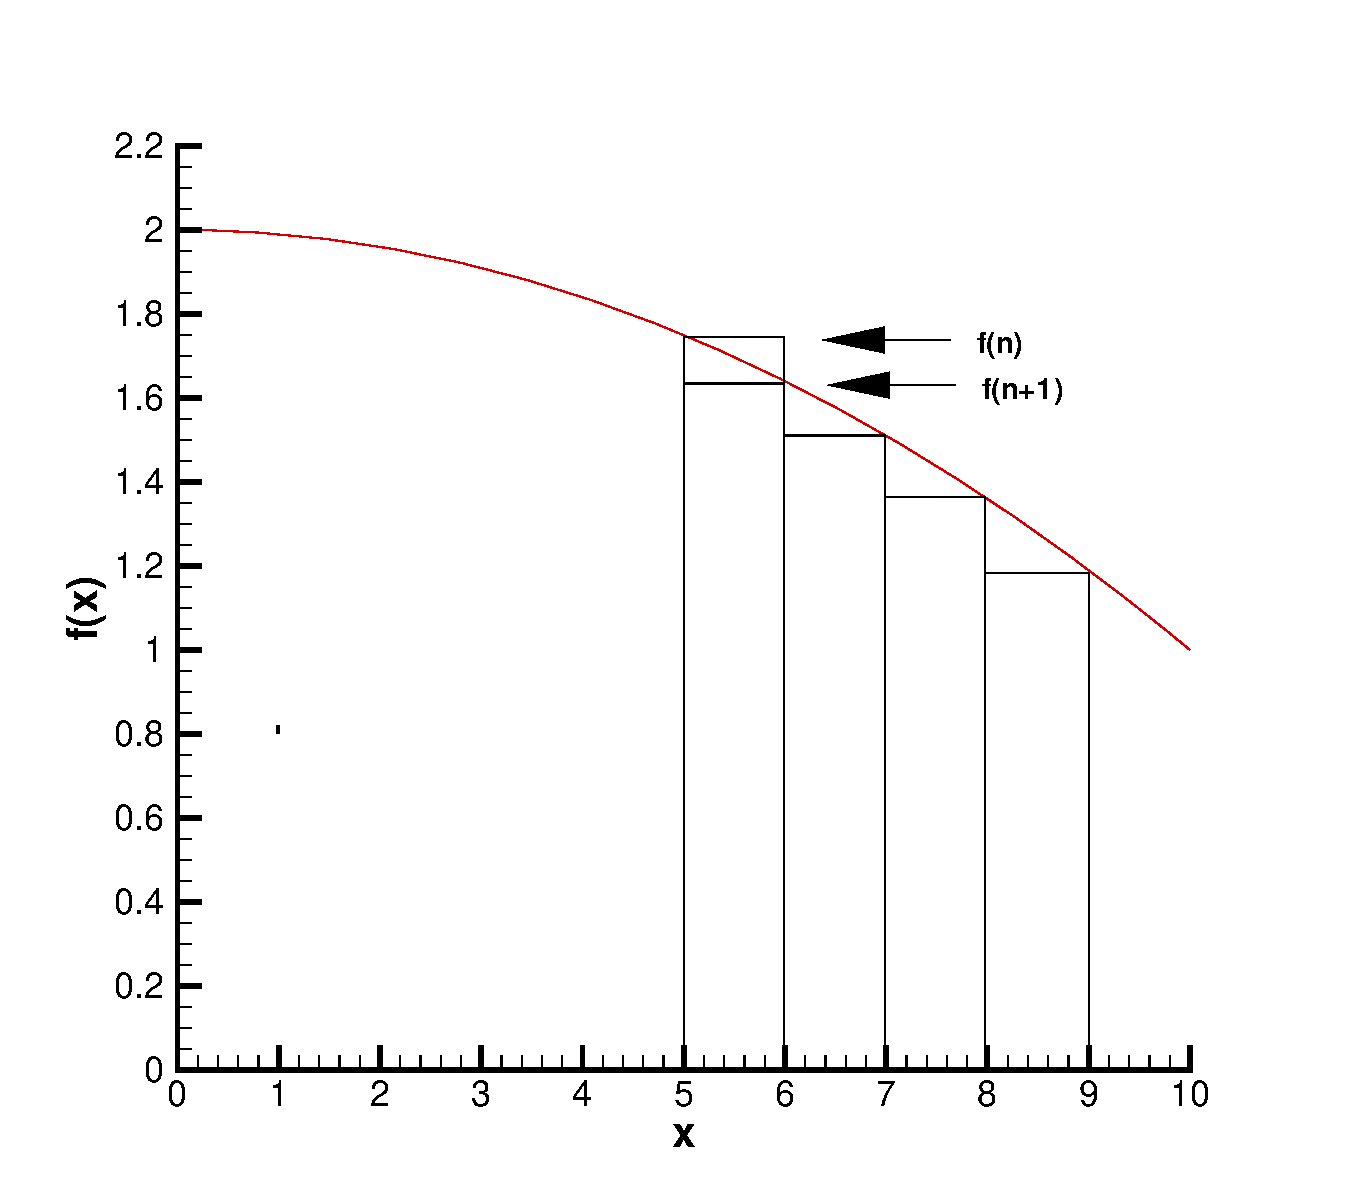
\includegraphics[width= 0.9\textwidth]{Figures/tecplot/snb.pdf}
%	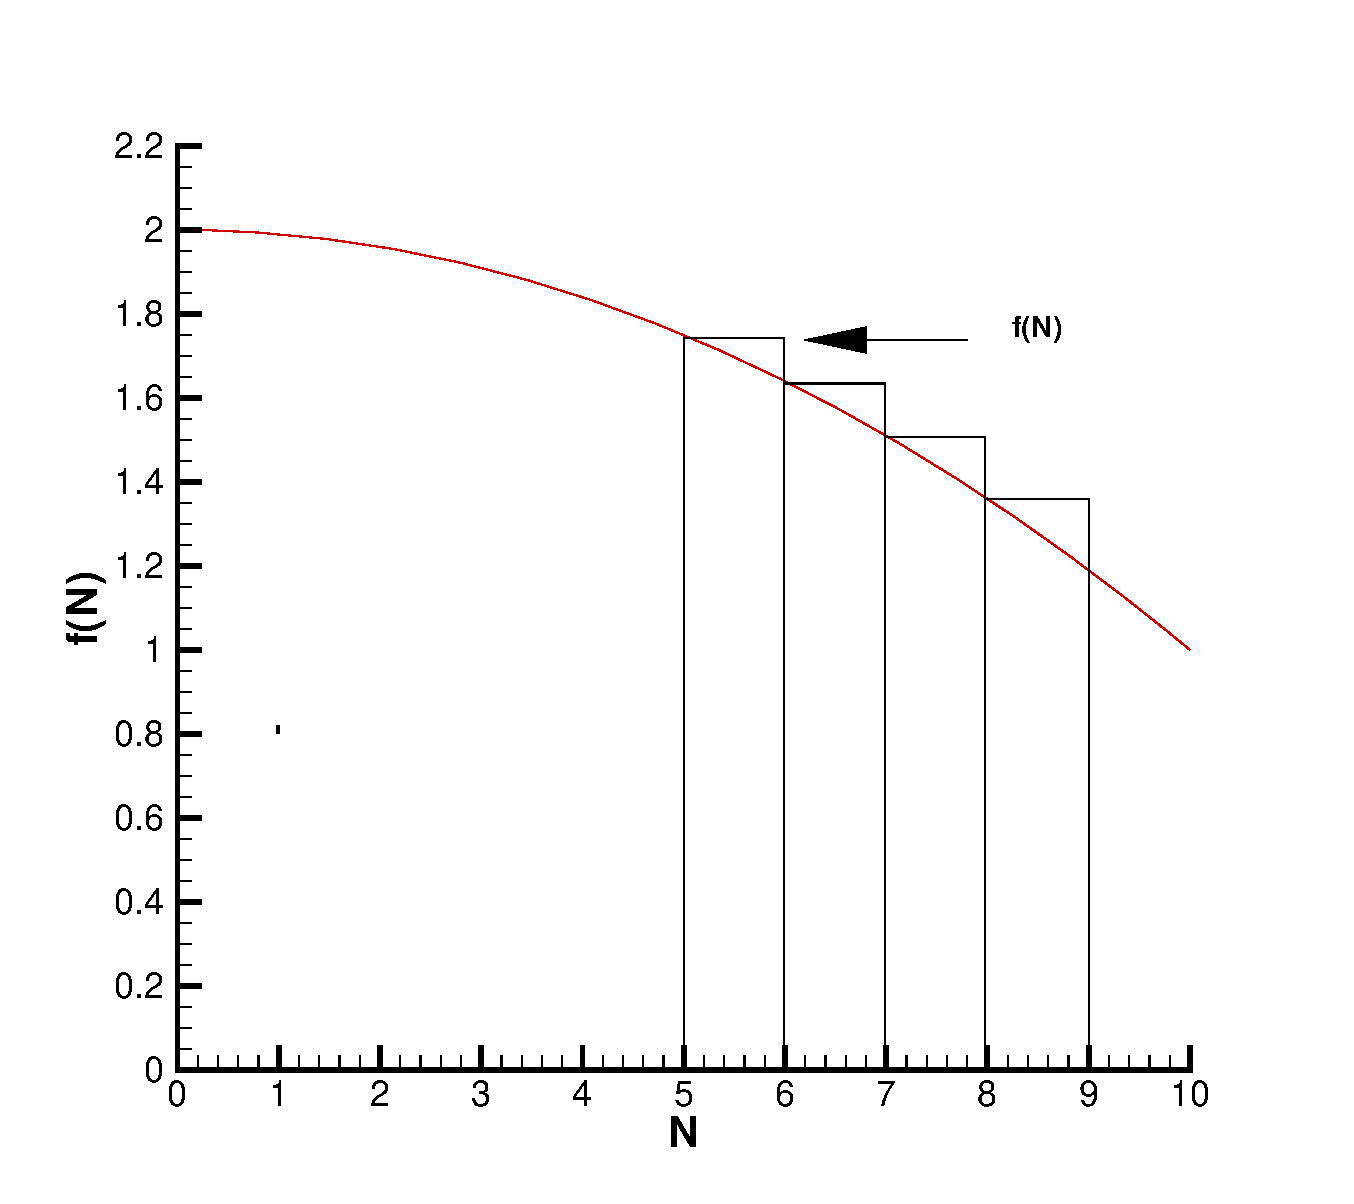
\includegraphics[width= 0.49\textwidth]{Figures/tecplot/sn.pdf}
	\caption{Relation between the integral of $ f:  \mathbb{R} \rightarrow \mathbb{R} $ and a sum of a numerical series with general term $ f : \mathbb{N} \rightarrow \mathbb{R}$.}
	\label{fig:sn}
\end{figure}



A generic $ f(x) $ function is represented in figure \ref{fig:sn}. Besides, the image of $ f(x) $ for different natural values $ n $ of the independent variable $ x $ is plotted. Rectangles of height $ f(n)$ and base one are represented in the same figure.  
From figure  \ref{fig:sn}, the integral from $ n $ and $ n+1 $ can be bounded by the area of two rectangles of height $ f(n+1) $ and $ f(n) $ by the following expression:
$$
f(n) \le \ \int _{n} ^{n+1}  f(x) \ dx \le \ f(n+1) 
$$

A lower bound for the rest $ S -S_N $ is given by:  
$$
S-S_N = \sum_{n=N+1} ^\infty f(n) \le \sum_{N+1}  ^\infty \int _{n} ^{n+1}  f(x) \ dx = 
\int _{N+1} ^{\infty}  f(x) \ dx
$$
Un upper bound is given by: 
$$
S-S_N = \sum_{n=N} ^\infty f(n+1) \ge \sum_{N}  ^\infty \int _{n} ^{n+1}  f(x) \ dx = 
\int _{N} ^{\infty}  f(x) \ dx
$$


With these bounds, the rest $ S- S_N $ can be bounded by the following expression: 
$$
\int _{N+1} ^{\infty}  f(x) \ dx\  \le \ S -S_N \ \le \int _{N} ^{\infty}  f(x) \ dx
$$

\newpage
 \listings{\home/Sum_series.f90}{real function Summation_2n}
          {end function}{Sum_series.f90}


\newpage
 \listings{\home/Sum_series.f90}{real function Summation_factorialn}
          {end function}{Sum_series.f90}

\label{numeric_series}

%Dar el resultado de la suma de los 100 primeros t�rminos de las siguientes series: 
%\begin{enumerate}    
%	\item Serie de n�meros naturales.
%	\item Serie de n�meros naturales impares.
%	\item Serie num�rica donde el t�rmino general de la serie es: $ a_n = 1/n^2 $ desde $ n= 1 $.  
%	\item Serie num�rica donde el t�rmino general de la serie es $ a_n = 1/ n! $ desde $ n=1$.  % e 
%	\item Serie num�rica donde el t�rmino general de la serie es
%	$ a_n = (-1)^{n+1}/ (2n-1) $ desde $ n=1$.   
%\end{enumerate}         





%___________________________________________________________________________________________________
\newpage 
\section{Convergence rate} 
One of the main focus of the numerical approximation techniques is to attain expansions with high rate of convergence. When dealing with numerical series, it is desirable to obtain a precise  result by adding the smallest number ot terms to reduce CPU time. 
However, the number of terms to obtain the precise accuracy depends on the convergence rate of the series.
In other words, the behavior of $ a_n $ con $ n \rightarrow \infty $ defines the number of terms to be added. 



Algebraic spectral or exponential convergence 

 \unitlength 0.8mm
\begin{center}
	\begin{figure}[htbp]
		\centering
		\vbox{
			\begin{picture}(120,85)
			
			%   \put(0,0){\framebox(120,85)}
			
			\drawline [200](40,70)(80,50)               
			\drawline [200](40,65)(80,35) 
			\drawline [200](40,60)(80,20)           
			
			\put(30,10){\vector(0,1){70}}
			\put(30,10){\vector(1,0){70}}   
			
			\put(10,78){$\log{|a_{n}|}$}                                        
			\put(90,5){$\log{n}$}
			\put(85,35){Algebraic ($q $)}            
			
			\put(38,20){Spectral}    
			
			\qbezier(40,55)(55,40)(60,10)
			
			\qbezier(90,60)(90,40)(70,20)
			
			\put(70,20){\vector(-1,-1){0}}          
			
			
			
			\end{picture} 
			\caption{Convergence of $ a_n $ with $ n $.  Algebraic and spectral  convergence. }
		}
	\end{figure}
\end{center}



%___________________________________________________________________________________________________
\newpage 
\section{Vectorial operations with vectors and matrices} 



Considerar los vectores 
$V, W \in \mathbb{R}^N$ 
de componentes: 

$$
\{ v_i =\frac{1}{i^2}, \ \ i = 1 \ldots  N \},
$$

$$
\{ w_i = \frac{(-1)^{i+1}}{2i-1}, \ \ i = 1 \ldots  N \}.
$$






Considerar la matriz $ A \in { \cal{M}}_{N \times N} (\mathbb{R})$ 
%donde su t�rmino gen�rico vale %$ a_{ij} = (i/N)^j $.
 
%Escribir un programa para calcular  las operaciones siguientes con $N=100$: 
%\begin{enumerate}
%	\item Suma de  todas las componentes del vector $V$ y del vector $ W$. 
%	\item Suma de  todas las componentes de la matriz $A$.   
%	\item Suma de  las componentes del vector $W$ mayores que cero.
%	\item Producto escalar de los vectores $V$ y $W$.   
%	\item Producto escalar del vector $V$ y la columna $N$ de la matriz $A$. 
%	\item Suma de las componentes de vector que resulta de  multiplicar la matriz $A$ por el vector $V$.
%	\item Traza de la matriz $A$.
%\end{enumerate}

\newpage

 \listings{\home/Matrix_operations.f90}{subroutine Examples_matrix_operations}
          {end subroutine}{Matrix_operations.f90}


\newpage 

 \listings{\home/Matrix_operations.f90}{real function my_dot_product}
{end function}{Matrix_operations.f90}



%_______________________________________________________________________________________________
\newpage  
\section{Dynamic allocation} 



%Dada la matriz  $A \in {\cal M}_{M \times M} (\mathbb{R})$  de t�rmino gen�rico 
$$
\{ a_{ij} = (i/M)^j, \ \ i=0, \ldots M-1, \ \  j=0, \ldots M-1 \}. 
$$
calcular las siguientes operaciones: 


\begin{enumerate}	
	\item Calcular 
	$$  \sum_{M=1} ^{10} traza(A) $$ 
	\item Calcular 
	$$  \sum_{M=1} ^{5} traza(A^2) $$ 
	\item Calcular  con $ M=4 $
	$$  traza \left( \sum_{k=1} ^{5} A^k  \right) $$
\end{enumerate}     





%\lstinputlisting[language=Fortran, firstline=10, lastline=50, caption = \mycap{Dynamic_allocation.f90} ]{\home/sources/Dynamic_allocation.f90}

%\newpage
%\lstinputlisting[language=Fortran, firstline=50,lastline=85, caption = \mycap{Dynamic_allocation.f90} ]{\home/sources/Dynamic_allocation.f90}

\newpage

 \listings{\home/Dynamic_allocation.f90}{subroutine Matrices_allocation}
{end subroutine}{Dynamic_allocation.f90}


\newpage 
%___________________________________
\section{Piece-wise functions} 
%___________________________________

\listings{\home/Piecewise_functions.f90}{elemental real function}
{end function}{Piecewise_functions.f90}


\newpage
\listings{\home/Piecewise_functions.f90}{subroutine Function_examples}
{end subroutine}{Piecewise_functions.f90}

 
  
  
  
  
  
  
  \newpage
  %__________________________________________
  \section{Series expansion} 
  %_________________________________________
  
  One of the main focus of numerical methods is to approximate functions by means of different expansions: 
  \begin{enumerate} 
  	\item Polynomial expansion: Taylor, Lagrange 
  	\item Trigonometric series: sine and cosine expansions. 
  	\item Expasion by means of known basis:  Chebyshev, Legendre,.. 
  \end{enumerate} 
  The same function can be expanded or approximated with different basis.
  It goes without saying that the computer only allows to sum a finite number $ N $  of terms. 
  
  Hence, the best election is related to the rate of convergence 
  of the expansion. In other words, given a tolerance error between the approximation and the exact function, the best expansion allows to obtain the approximation with a minimum number of terms $N$. 
  
  
  \section{Parseval identity} 
  
  \begin{equation} 
  f ( x)  =  \sum_{k=-\infty} ^{\infty}  \hat{c}_k  e^{ i k x }
  \end{equation} 
  
  \begin{equation} 
  f ( x)  =  \sum_{k=0} ^{\infty} \  \hat{a}_k  \ \cos k x + \sum_{k=1} ^{\infty} \  \hat{b}_k  \sin k x
  \end{equation} 	
  
  \begin{equation} 
  \hat{c}_k  =  \frac{1}{2} \ ( \ \hat{a}_k  - i \ \hat{b}_k \ ),  \quad k=1, \ldots, N/2. 
  \end{equation}	
  
  \begin{equation} 
  \hat{c}_{-k}  =  \overline{ \hat{c}} _{k}  , \quad k=1, \ldots, N/2. 
  \end{equation} 	
  
  
  \begin{equation} 
  \int _{-\pi} ^{\pi} f(x)^2 \ dx = 2 \pi \left(    | \hat{c}_0 |^2 + 2 \sum_{k=1} ^{\infty} |  \hat{c}_k  |^2 \right) 
  \end{equation} 
  
  Let $ f(x) = x $ $ \forall x \in [-\pi, +\pi ] $ and extend $ f(x) $  periodically to the right and to the left. Once $ f(x) $ is defined in this way, it can be approximated by a sine expansion: 
  \begin{equation} 
  f ( x)  =  \sum_{k=1} ^{N/2} \   \hat{b}_k  \sin k x, 
  \end{equation} 
  where the coefficients $ \hat{b}_k $ are given by:
  \begin{equation} 
  \hat{b}_k   = \frac{ (-1)^{k+1} }{ \pi k }, \qquad k=1, \ldots, N/2. 
  \end{equation} 
  
  Using Parseval identify with $ f(x)$, the following  summation is obtained: 
  \begin{equation} 
  \sum_{k=1} ^{\infty} \  \frac{1}{n^2}  \  = \frac{\pi^2}{6}
  \end{equation} 
  
  
  
  
  Aproximar  mediante un desarrollo en serie de potencias de la forma
  \[  f(x) = \sum_{k=0} ^M a_k \  x^k, \qquad \qquad a_k = \frac{  f^{(k)} (0)  }{ k! },  \]  
  las funciones $f : \mathbb{R} \rightarrow \mathbb{R}$, siguientes:    
  \begin{enumerate}
  	\item $f(x) = e^x$ y calcular el valor $ f(1) $ con $ M=5$.      
  	\item $f(x) = \sin(x)$ y calcular el valor $ f(\pi/2)$  con $M=8$.      
  	\item $f(x) = \cosh(x)$ y calcular el valor $ f(1) $  con $M=10$. 
  	\item $f(x) = \displaystyle \frac{1}{1 - x}$ y calcular el valor $ f(0.9) $  con $M=20$.  
  	%	\item $f(x) = e^x $ y calcular el valor m�s preciso de  $ f(1) $ con doble precisi�n.        
  	%	\item $f(x) = \sin(x)$ y calcular el valor m�s preciso  $ f(\pi/2)$ con doble precisi�n.   
  	%	\item $f(x) = \cosh(x)$ y calcular el valor m�s preciso de  $ f(1) $ con doble precisi�n.
  	%	\item $f(x) = \displaystyle \frac{1}{1 - x}$ y calcular el valor  m�s preciso de $ f(0.9) $ con doble precisi�n.
  	
  \end{enumerate}
  
  \newpage 
  
  \listings{\home/Series_expansion.f90}{subroutine Expansion_examples}
  {end subroutine}{Series_expansion.f90}
  
  \newpage
  \listings{\home/Series_expansion.f90}{abstract interface}
  {end interface}{Series_expansion.f90}
  
  
  \newpage
  \listings{\home/Series_expansion.f90}{real function expansion}
  {end function}{Series_expansion.f90}
  
  
  
  \newpage   
  \listings{\home/Series_expansion.f90}{real function fk_sin}
  {end function}{Series_expansion.f90}
  
  
  
  \newpage   
  \listings{\home/Series_expansion.f90}{Convergence_examples}
  {end subroutine}{Series_expansion.f90}  
  
  
  
  
  
  
  
  
  
  \newpage   
  \section{Read an external file} 

  
  \listings{\home/read_files.f90}{subroutine Test_load_matrix}
  {end subroutine}{read_files.f90}
  
  \newpage 
  \listings{\home/read_files.f90}{function load_matrix}
  {end function}{read_files.f90}
  
  \newpage
  \listings{\home/read_files.f90}{function columns}
  {end function}{read_files.f90}
  
  
  
  
  
  
 %   A batch file named: \mycap{Preliminary_examples.bat} allows to compile and to run this main program.  
 
 
 % \newpage  
 
 
 
 
 %   \subsection{Windows}
 
 
 % _______________ RUN EXAMPLES_________________________________________________
 
 %   >compile_Cauchy_Problem_examples.bat
 %   
 %   >compile_BVP_examples.bat 
 %   
 %   >
 %   
 %   >
 %   
 %   
 %   
 %   Examples of use compile.bat 
 %   
 % %  _________BASIC USAGE___________________________________________________________ 
 %   
 % %  >compile main 
 %   
 %   The file main.f90 contains the main program to be executed
 %   
 %%   e.g. to compile and to execute the "hello world" first example 
 %   
 %   >compile main    
 %   
 %   
 % %  ___________ADVANCED USER______________________________________________________
 %   
 %   If the user develops a new module, or he wants to use existing examples,
 %   the compilation procedure is as follows: 
 %   
 %%   > compile module_name main 
 %   
 %   1) module_name is a fortran module file which is located in sources. 
 %   
 %   2) main file is the main program.
 %   It contains a use setence to access module_name and it calls some subrutine of  the module 
 %   
 %   
 %   e.g. 
 %   > compile 
 %   
 
 
 
 
 
 
 %   
 %   
 %   
 %   
 %   Informatics 2017/2018 Aerospace Engineering (UPM) 
 %   
 %   How to install FORTRAN and graphical windows in windows 10 
 %   
 %   Author: Juan A. Hernandez:  juanantonio.hernandez@upm.es 
 %   
 %   
 %   
 %   %   A) Copy Informatica\_2018 to Desktop 
 %   
 %   B) Check the compiler 
 %   1)open command prompt and type >compile Hello\_world
 %   2)open  command prompt and type >compile plot\_graph
 %   
 %   
 %   \subsection{Ubuntu}
 %   
 %   
 %   
 %   Informatics 2017/2018 Aerospace Engineering (UPM) 
 %   
 %   How to install FORTRAN and graphical windows in Ubuntu from windows 10 
 %   
 %   Author: Juan A. Hernandez:  juanantonio.hernandez@upm.es 
 %   
 %   
 %   
 %   
 %   A) Install UBUNTU from Windows 10 (skip this step if your machine is UBUNTU) 
 %   
 %   1) Setting/Security/Developer ( allow to create and modify programs ) 
 %   
 %   2) control panel/programs/Windows characteristics allow UBUNTU 
 %   
 %   3) cmd> bash . Create user and password UBUNTU machine 
 %   
 %   4) Install X11 server for graphical windows ( XMing ) to run graphical linux binaries from shell.
 %   Capability to start 64-bit GUI-programs from the desktop file manager 
 %   
 %   5) Install graphical vim editor to check: 
 %   
 %   \$sudo apt-get install vim-gtk
 %   
 %   Now, you?ll need to set the ?DISPLAY? environment variable to point at the X server running on your Windows 10 PC. 
 %   If you don?t do this, graphical applications will simply fail to launch.
 %   To do this, run the following command in the Bash environment:
 %   
 %   \$export DISPLAY=:0
 %   \$gvim
 %   
 %   
 %   B) Install gfortran 
 %   
 %   1) \$ sudo apt-get install gfortran 
 %   
 %   
 %   
 %   C) Install DISLIN to plot with UBUNTU 
 %   
 %   1)  should install OpenMotif on Ubuntu 
 %   
 %   
 %   \$ sudo add-apt-repository deb http://archive.ubuntu.com/ubuntu lsb\_release -sc universe multiverse
 %   
 %   \$ sudo apt-get update 
 %   
 %   \$ sudo apt-get install libxm4
 %   
 %   \$ sudo apt-get install libmotif4* libmotif-dev
 %   
 %   \$sudo apt-get install libx11-dev libxt-dev libgl1-mesa-dev  WARNING:(l1 ele and then one )
 %   
 %   
 %   2) Check the compiler 
 %   
 %   1)\$ ./compile.sh Hello\_world
 %   2)\$ ./compile.sh plot\_graph
 %   
 %   
 %   
 %   \subsection{MAC} 
 %   
 %   Informatics 2017/2018 Aerospace Engineering (UPM) 
 %   
 %   How to install FORTRAN and graphical windows in MAC OS 
 %   
 %   Author: Juan A. Hernandez:  juanantonio.hernandez@upm.es 
 %   
 %   
 %   1) How to execute a Terminal 
 %   
 %   Applications/ Utilities/ Terminal
 %   
 %   2) How to execute a Terminal in a specific folder
 %   
 %   System Preferences/ Keyboard/ Speed functions/ Services - scroll and select "Terminal in the folder"
 %   
 %   
 %   
 %   3) Install gFortran to compile
 %   
 %   3.1) Install manager HOMEBREW (https://brew.sh)
 %   3.2) \$ brew install gcc
 %   
 %   
 %   4) Install Openmotiff
 %   
 %   4.1) Install server X11 through XQuartz (https://www.xquartz.org)
 %   Capability to start 64-bit GUI-programs using x-windows from the shell 
 %   
 %   4.1)\$ brew install openmotif
 %   
 %   
 
 
 
 
 
 
 
   
   
   
   
    
    
    
    
    
    
    
   
   
